\documentclass[a4paper,10pt,twoside,openany]{book}

\usepackage[lang=hebrew]{maths}
\usepackage{hebrewdoc}
\usepackage{stylish}
\usepackage{lipsum}
\let\bs\blacksquare

\setlength{\parindent}{0pt}

%%%%%%%%%%%%
% Styling %
%%%%%%%%%%%%

\usepackage{enumitem}

%%%%%%%%%%%%%
% Counters  %
%%%%%%%%%%%%%

\setcounter{section}{1}     
            
%BIBLIOGRAPHY
\usepackage[
backend=biber,
style=alphabetic,
]{biblatex}
\addbibresource{bibliography.bib} %Imports bibliography file

\title{
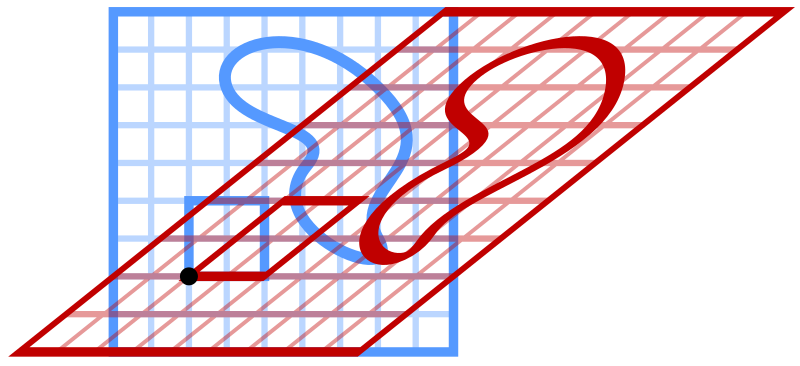
\includegraphics[width=6in]{images/front.png}\\
\vspace{30pt}
\Huge
מבוא לתורת המספרים (104157)
\\
אביב 2024
\\
רשימות תרגולים
\vspace{30pt}
\\
\huge
אלן סורני
\vspace{30pt}
\\
\Large
הרשימות עודכנו לאחרונה בתאריך ה־%
\today
}
\date{}

\begin{document}
\frontmatter
\maketitle
\tableofcontents

\mainmatter

\section*{סימונים}

\begin{itemize}
\item[-]
$\mbb{N} = \set{0, 1, 2, \ldots}$
אוסף המספרים הטבעיים.
\item[-]
$\mbb{N}_+ = \set{1, 2, 3, \ldots}$
אוסף המספרים הטבעיים החיוביים (כלומר, לא כולל אפס).
\item[-]
$\brs{n} = \set{1, \ldots, n}$.
\item[-]
$\floor{x}$
המספר הכי גדול שקטן או שווה ל־%
$x \in \mbb{R}$.
\item[-]
$\ceil{x}$
המספר הכי קטן שגדול או שווה ל־%
$x$.
\item[-]
\begin{align*}
\gcd\prs{a_1, \ldots, a_n} \\
\lcm\prs{a_1, \ldots, a_n}
\end{align*}
בהתאמה, המחלק המשותף הגדול ביותר של המספרים
$a_1, \ldots, a_n$,
והכפולה המשותפת המינימלית שלהם.
\end{itemize}

\chapter{תרגול 3 - שימושים בפריקות יחידה}

\section{תזכורת}

\begin{definition}
יהי
$n \in \mbb{N}_+$.
נגדיר
\begin{enumerate}
\item $\nu\prs{n} \coloneqq \sum_{d \mid n} 1$. זה מספר המחלקים של $n$.
\item $\sigma\prs{n} \coloneqq \sum_{d \mid n} d$. זה סכום המחלקים של $n$.
\item \[\text{.}\phi\prs{n} \coloneqq \sum_{\substack{\gcd\prs{d,n} = 1 \\ 1 < d < n}} 1\] זה מספר המספרים הטבעיים שקטנים מ־%
$n$
וזרים לו.
זאת נקראת
\textbf{פונקציית אוילר (\textenglish{Euer totient function})}.
\item $\pi\prs{n}$ מספר האיברים הראשוניים הקטנים או שווים ל־%
$n$.
זאת נקראת
\textbf{פונקציית המספרים הראשוניים (
\textenglish{prime-counting~function})}.
\item \[\mu\prs{n} = \begin{cases}
\prs{-1}^\ell & \text{\textenglish{$\forall p$ prime}}: p^2 \nmid n \\
0 & \text{otherwise}
\end{cases}\]
כאשר
$\ell$
מספר הראשוניים שמחלקים את
$n$.
זאת נקראת
\textbf{פונקציית מביוס (\textenglish{Möbius function})}.
\end{enumerate}
\end{definition}

\section{תרגילים}

\begin{exercisechap}[פרק 2, תרגיל 7]
הסיקו מתרגיל 6 כי
\[\ord_p\prs{n!} \leq \frac{n}{p-1}\]
וכי
\[\text{.} \sqrt[n]{n!} \leq \prod_{p \mid n!} p^{1 / \prs{p-1}}\]
\end{exercisechap}

\begin{solution}
לפי תרגיל 6 מהתרגול הקודם,
\begin{align*}
\text{.} \ord_p\prs{n!} &= \sum_{k = 1}^{\infty} \floor{\frac{n}{p^k}}
\end{align*}
נקבל כי
\begin{align*}
\ord_p\prs{n!} &\leq \sum_{k=1}^{\infty} \frac{n}{p^k}
\\&= n \sum_{k=1}^{\infty} \prs{\frac{1}{p}}^k
\end{align*}
וכיוון ש־%
$p \in \mbb{N}_+$
ראשוני מתקיים
$\abs{\frac{1}{p}} < 1$.
מסכום סדרה הנדסית נקבל כי
\begin{align*}
\sum_{k=1}^{\infty} \prs{\frac{1}{p}}^k
\\&= \frac{1 - \prs{1 - \frac{1}{p}}}{1 - \frac{1}{p}} - 1
\\&= \frac{\frac{1}{p}}{1 - \frac{1}{p}}
\\&= \frac{1}{p - 1}
\end{align*}
ולכן
\[\text{.}\ord_p\prs{n!} \leq \frac{n}{p - 1}\]

אז מתקיים גם
\begin{align*}
n! &= \prod_{\substack{p \mid n \\ \text{\textenglish{$p$ prime}}}} p^{\ord_p\prs{n!}}
\\&\leq
\prod_{\substack{p \mid n \\ \text{\textenglish{$p$ prime}}}} p^{\frac{n}{p-1}}
\\&\leq
\prod_{p \mid n} p^{\frac{n}{p-1}}
\\&=
\prs{\prod_{p \mid n} p^{\frac{1}{p-1}}}^n
\end{align*}
ולכן
\[\text{,} \sqrt[n]{n!} \leq \prod_{p \mid n} p^{\frac{1}{p-1}}\]
כנדרש.
\end{solution}

\begin{exercisechap}[פרק 2, תרגיל 8]
השתמשו בתוצאת התרגיל הקודם כדי להראות שיש אינסוף ראשוניים.

\emph{רמז:}
הראו קודם שמתקיים
$\prs{n!}^2 \geq n^n$
לכל
$n \in \mbb{N}_+$.
\end{exercisechap}

\begin{solution}
ראשית, נראה כי
$\prs{n!}^2 \geq n^n$
לכל
$n \in \mbb{N}_+$.

מתקיים
\begin{align*}
n! &= \prod_{k=0}^{n-1} \prs{k + 1} \\
n! &= \prod_{k=0}^{n-1} \prs{n - k}
\end{align*}
ולכן
\begin{align*}
\text{.} \prs{n!}^2 = \prod_{k=0}^{n-1} \prs{k+1}\prs{n-k}
\end{align*}

נראה כי הגורמים הנסכמים גדולים או שווים ל־%
$n$.
כאשר
$k = 0$
מתקיים
$\prs{k+1}\prs{n-k} = n$.
כאשר
$0 < k \leq \frac{n}{2}$
מתקיים
$n - k \geq \frac{n}{2}$
ואז
\[\text{.}\prs{k+1} \prs{n-k} \geq \frac{\prs{k+1} n}{2} \geq \frac{2n}{2} = n\]
כאשר
$\frac{n}{2} < k < n-1$
נקבל כי
$n - k \geq 2$
ולכן
\[\text{.} \prs{k+1}\prs{n-k} > 2 \cdot \frac{n}{2} = n\]
כאשר
$k = n-1$
נקבל
\[\text{.} \prs{k+1}\prs{n-k} = \prs{n-1+1} \cdot \prs{n-n+1} = n \cdot 1 = n\]
לכן
$\prs{n!}^2 \geq \prod_{k=0}^{n-1} n = n^n$,
כנדרש.

כעת, מהוכחת הסעיף הקודם ניתן לראות כי
\begin{align*}
\sqrt[n]{n!} \leq \prod_{\substack{p \mid n! \\ \text{\textenglish{$p$ prime}}}} p^{\frac{1}{p-1}}
\end{align*}
ואם נראה שאגף שמאל שואף לאינסוף נקבל שגם אגף ימין שואף לאינסוף, ובפרט שיש אינסוף ראשוניים.

אכן, מכך שמתקיים
$\prs{n!}^2 \geq n^n$
נובע כי
$\sqrt[n]{n!} \geq \sqrt{n}$
ולכן
$\lim_{n\to\infty}\sqrt[n]{n!} = \infty$.
\end{solution}

\begin{exercisechap}[פרק 2, תרגיל 15]
הראו כי
\begin{enumerate}[label = (\alph*)]
\item לכל
$n \in \mbb{N}_+$
מתקיים
\[\text{.} \sum_{d \mid n} \mu\prs{n/d} \nu\prs{d} = 1\]
\item לכל
$n \in \mbb{N}_+$
מתקיים
\[\text{.} \sum_{d \mid n} \mu\prs{n/d} \sigma\prs{d} = n\]
\end{enumerate}
\end{exercisechap}

\begin{solution}
ראשית נזכיר כי
\begin{align*}
\prs{f * g}\prs{n} \coloneqq \sum_{d \mid n} f\prs{d} g\prs{\frac{n}{d}}
\end{align*}
לכל
$f,g \colon \mbb{N}_+ \to \mbb{C}$,
וכי ראינו שלכל
$f$
כנ"ל מתקיים
$f = \prs{f * 1} * \mu$.

\begin{enumerate}[label = (\alph*)]
\item
מתקיים
\[\text{,} \sum_{d \mid n} \mu\prs{n/d} \nu\prs{d} = \prs{\nu * \mu}\prs{n}\]
ונשים לב כי
\[\text{.} \nu\prs{n} = \sum_{d \mid n} 1 = \prs{1 * 1}(n)\]
אז
\begin{align*}
\text{,} \prs{\nu * \mu}\prs{n} = \prs{1 * 1 * \mu}\prs{n} = 1\prs{n} = 1
\end{align*}
כנדרש.

\item
מתקיים
\begin{align*}
\text{,} \sum_{d \mid n} \mu\prs{n/d} \sigma\prs{d} = \prs{\sigma * \mu}\prs{n}
\end{align*}
ונשים לב כי
\[\text{.} \sigma\prs{n} = \sum_{d \mid n} d = \prs{\id_{\mbb{N}_+} * 1}\prs{n}\]
אז
\begin{align*}
\text{,} \prs{\sigma * \mu}\prs{n} = \prs{\id_{\mbb{N}_+} * 1 * \mu}\prs{n} = \id_{\mbb{N}_+}\prs{n} = n 
\end{align*}
כנדרש.
\end{enumerate}
\end{solution}

\begin{exercisechap}[פרק 2, תרגיל 16]
הראו כי
$\nu\prs{n}$
אי־זוגי אם ורק אם
$n$
ריבוע.
\end{exercisechap}

\begin{solution}
נכתוב
$n = \prod_{i \in \brs{k}} p_i^{r_i}$.
ראינו כי אז
\[\text{.}\nu\prs{n} = \prod_{i \in \brs{k}} \prs{r_i + 1}\]
מספר זה אי־זוגי אם ורק אם כל ה־%
$r_i$
זוגיים, מה שמתקיים אם ורק אם
$n$
ריבוע.
\end{solution}

\begin{exercisechap}[פרק 2, תרגיל 16]
הראו כי
$\sigma\prs{n}$
אי זוגי אם ורק אם
$n$
ריבוע או ריבוע כפול
$2$.
\end{exercisechap}

\begin{solution}

\end{solution}

\begin{exercisechap}[פרק 2, תרגיל 18]
הראו כי
\[\text{.} \forall m,n \in \mbb{N}_+ : \phi\prs{n} \phi\prs{m} = \phi\prs{\gcd\prs{n,m}} \phi\prs{\lcm\prs{n,m}}\]
\end{exercisechap}

\begin{solution}
נזכיר כי עבור
$x = p_1^{a_1} \cdot \ldots p_{\ell}^{a_{\ell}}$
מתקיים באופן כללי
\[\text{.} \phi\prs{x} = x \prod_{k \in \brs{\ell}} \prs{1 - \frac{1}{p_k}}\]

יהיו
\begin{align*}
n &= \prs{\prod_{i \in \brs{k}} p_i^{\alpha_i}} \prs{\prod_{i \in \brs{\ell}} q_i^{r_i}} \\
m &= \prs{\prod_{i \in \brs{k}} p_i^{\beta_i}} \prs{\prod_{i \in \brs{\tilde{\ell}}} \tilde{q}_i^{s_i}}
\end{align*}
הפירוקים של
$n,m$
לראשוניים, כאשר
$p_1, \ldots, p_k$
הראשוניים שמחלקים גם את
$n$
וגם את
$m$.

אז
\begin{align*}
\phi\prs{n} &= n \prs{\prod_{i \in \brs{k}} \prs{1 - \frac{1}{p_i}}} \prs{\prod_{i \in \brs{\ell}} \prs{1 - \frac{1}{q_i}}}
\\
\phi\prs{m} &= m  \prs{\prod_{i \in \brs{k}} \prs{1 - \frac{1}{p_i}}} \prs{\prod_{i \in \brs{\tilde{\ell}}} \prs{1 - \frac{1}{\tilde{q}_i}}}
\\
\phi\prs{\gcd\prs{n,m}} &= \gcd\prs{n,m} \prod_{i \in \brs{k}} \prs{1 - \frac{1}{p_i}}
\\
\phi\prs{\lcm\prs{n,m}} &= \lcm\prs{n,m} \prs{\prod_{i \in \brs{k}} \prs{1 - \frac{1}{p_i}}} \prs{\prod_{i \in \brs{\ell}} \prs{1 - \frac{1}{q_i}}} \prs{\prod_{i \in \brs{\tilde{\ell}}} \prs{1 - \frac{1}{\tilde{q}_i}}}
\end{align*}
וכיוון ש־%
$\gcd\prs{n,m} \lcm\prs{n,m} = nm$,
נקבל כי
\[\text{,}\phi\prs{n} \phi\prs{m} = \phi\prs{\gcd\prs{n,m}} \phi\prs{\lcm\prs{n,m}}\]
כנדרש.
\end{solution}

\chapter{תרגול 4 - עוד פריקות יחידה, וחשבון מודולרי}

\begin{exercisechap}[פרק 2, תרגיל 19]
הראו כי
\[\text{.} \forall m,n \in \mbb{N}_+ : \phi\prs{mn} \phi\prs{\gcd\prs{m,n}} = \gcd\prs{m,n} \phi\prs{m} \phi\prs{n}\]
\end{exercisechap}

\begin{solution}
כיוון שראשוני מחלק את
$mn$
אם ורק אם הוא מחלק את
$\lcm\prs{m,n}$,
נקבל כי
\begin{align*}
\frac{\phi\prs{mn}}{mn} &= \prod_{\substack{p \mid mn \\ \text{\textenglish{$p$ prime}}}} \prs{1 - \frac{1}{p}}
\\&=
\prod_{\substack{p \mid \lcm\prs{m,n} \\ \text{\textenglish{$p$ prime}}}} \prs{1 - \frac{1}{p}}
\\&=
\frac{\phi\prs{\lcm\prs{m,n}}}{\lcm\prs{m,n}} \text{.}
\end{align*}
נקבל כי
\begin{align*}
\phi\prs{mn} &= \frac{mn}{\lcm\prs{m,n}} \cdot \phi\prs{\lcm\prs{m,n}}
\\ \text{.}\hphantom{\phi\prs{mn}} &= \gcd\prs{m,n} \phi\prs{\lcm\prs{m,n}}
\end{align*}
לכן
\begin{align*}
\phi\prs{mn} \phi\prs{\gcd\prs{m,n}} &= \gcd\prs{m,n} \phi\prs{\lcm\prs{m,n}} \phi\prs{\gcd\prs{m,n}}
\\&= \gcd\prs{m,n} \phi\prs{m} \phi\prs{n}
\end{align*}
כאשר בשוויון השני השתמשנו בתרגיל הקודם.
\end{solution}

\begin{exercisechap}[פרק 2, תרגיל 20]
הראו כי
\[\text{.} \prod_{d \mid n} d = n^{\nu\prs{n} / 2}\]

היעזרו בעובדה הבאה:
$\nu\prs{n}$
אי־זוגי אם ורק אם
$n$
ריבוע.
\end{exercisechap}

\begin{solution}
יהי
$n = \prod_{i \in \brs{k}} p_i^{r_i}$
פירוק של
$n$
לראשוניים.

נניח ראשית כי
$n = m^2$
עבור
$m \in \mbb{N}_+$.
מתקיים
\[\text{.} n^{\nu\prs{n} / 2} = \prs{m^2}^{\nu\prs{n} / 2} = m^{\nu\prs{n}}\]
אז
\[\text{,} \ord_{p_i} \prs{ n^{\nu\prs{n}/2} } = \nu\prs{n} \cdot \ord_{p_i}\prs{m}\]
ולכן די להראות כי
\[\text{.} \ord_{p_i} \prs{\prod_{d \mid n}} = \nu\prs{n} \cdot \ord_{p_i}\prs{m}\]
כיוון ש־%
$m^2 = n$,
מתקיים
$\ord_{p_i}\prs{n} = 2 \ord_{p_i}\prs{m}$,
לכן
$\ord_{p_i}\prs{m} = \frac{\ord_{p_i}{n}}{2}$.
לכן די להוכיח כי
\[\text{.} \ord_{p_i} \prs{\prod_{d \mid n} d} = \frac{\nu\prs{n} \cdot \ord_{p_i}\prs{n}}{2}\]

אם
$n$
אינו ריבוע,
$\nu\prs{n}$
זוגי, ואז
$\nu\prs{n} / 2$
שלם. נקבל כי במקרה זה
\[\text{,}\ord_{p_i}\prs{n^{\nu\prs{n} / 2}} = \frac{\nu\prs{n} \cdot \ord_{p_i}\prs{n}}{2}\]
ולכן גם במקרה זה די להוכיח כי
\[\text{.} \ord_{p_i} \prs{\prod_{d \mid n} d} = \frac{\nu\prs{n} \cdot \ord_{p_i}\prs{n}}{2}\]

נקבע
$i \in \brs{k}$.
מתקיים
\begin{align*}
\text{.} \ord_{p_i} \prs{\prod_{d \mid n} d} = \sum_{d \mid n} \ord_{p_i}\prs{d}
\end{align*}
לכל
$r \in \set{0, \ldots, r_i}$
נסמן
\[\text{,} A_r = \set{d}{\substack{d \mid n \\ \ord_{p_i}\prs{d} = r}}\]
ואז
\begin{align*}
\text{.} \set{d}{d \mid n} &= \bigcup_{r = 0}^{r_i} A_r 
\end{align*}
כל הקבוצות
$A_r$
מאותו גודל, כי עבור בחירת החזקה עבור
$p_i$
יש אותו מספר דרכים לבחור את שאר החזקות.
מתקיים גם
$\abs{\bigcup_{r = 0}^{r_i} A_r} = \nu\prs{n}$,
ולכן
\[\abs{A_r} = \frac{\nu\prs{n}}{r_i + 1}\]
לכל
$r \in \set{0, \ldots, r_i}$.
נקבל
\begin{align*}
\sum_{d \mid n} \ord_{p_i}\prs{d} &=
\sum_{r \in \set{0, \ldots, r_i}} \sum_{d \in A_r} r
\\&=
\sum_{r \in \set{0, \ldots, r_i}} \abs{A_r} r
\\&=
\frac{\nu\prs{n}}{r_i + 1} \cdot \sum_{r \in \set{0, \ldots, r_i}} r
\\&= \frac{\nu\prs{n}}{r_i + 1} \cdot \frac{r_i \prs{r_i+1}}{2}
\\&= \frac{\nu\prs{n} r_i}{2}
\\&= \frac{\nu\prs{n} \ord_{p_i}\prs{n}}{2}
\end{align*}
כנדרש.

\end{solution}

\begin{exercisechap}[פרק 3, תרגיל 1]
הראו שיש אינסוף ראשוניים
$p$
עבורם
$p \equiv 5 \mod{6}$.
\end{exercisechap}

\begin{solution}
נניח בדרך השלילה שיש מספר סופי של ראשוניים
$p_1, \ldots, p_\ell$
עבורם
$p_i \equiv 5 \mod{6}$.

אם
$\ell$
אי־זוגי, נגדיר
$m = \prod_{i \in \brs{\ell}} p_i + 6$
ואז
\[m \equiv \prs{-1}^\ell \equiv -1 \mod{6}\]
וזה מספר שזר לכל
$p_i$.
אבל,
$ab \equiv -1 \mod{6}$
גורר שלפחות אחד מבין
$a,b$
שווה
$-1 \mod{6}$.
מפריקות יחידה, נקבל כי
$m$
חייב להתחלק בראשוני ששווה
$-1 \mod{6}$,
בסתירה לכך שהוא לא מתחלק באף
$p_i$.

אם
$\ell$
זוגי, נגדיר במקום זאת
$m = 5 \prod_{i \in \brs{\ell}} p_i + 6$
ונחזור למקרה הקודם.
\end{solution}

\begin{exercisechap}[פרק 3, תרגיל 6]
יהי
$n > 0$.
קבוצת מספרים
$\set{a_1, \ldots, a_{\phi\prs{n}}}$
נקראת
\textbf{מערכת שאריות מצומצמת מודולו $n$}
אם
$\gcd\prs{a_i, n} = 1$
לכל
$i \in \brs{\phi\prs{n}}$
וגם
$a_i \not\equiv a_j \mod{n}$
כאשר
$i \neq j$.

תהי
$R \coloneqq \set{a_1, \ldots, a_{\phi\prs{n}}}$
מערכת שאריות מצומצמת מודולו
$n$
ויהי
$a \in \mbb{Z}$
עבורו
$\gcd\prs{a,n} = 1$.
הראו כי
$aR \coloneqq \set{a a_1, \ldots, a a_{\phi\prs{n}}}$
מערכת שאריות מצומצמת מודולו
$n$.
\end{exercisechap}

\begin{solution}
ראשית, נשים לב כי לכל
$i \in \brs{\phi\prs{n}}$
מתקיים
$\gcd\prs{a a_i, n} = 1$
כי
$a, a_i$
שניהם זרים ל־%
$n$.

נסמן ב־%
$G \coloneqq \prs{\mbb{Z} / n \mbb{Z}}^\times$
את קבוצת השאריות מודולו
$n$
שזרות ל־%
$n$,
ונשים לב\textbackslash%
ניזכר שקבוצה זאת היא חבורה ביחס לכפל.
אכן, עבור
$x \in G$
כיוון שמתקיים
$\gcd\prs{x,n} = 1$
קיימים
$\alpha, \beta \in \mbb{Z}$
עבורם
$\alpha x + \beta n = 1$,
ואז
$\alpha x \equiv 1 \mod{n}$,
כלומר
$\alpha \equiv x^{-1} \mod{n}$.

בפרט, קיים איבר הופכי ל־%
$a$
מודולו
$n$,
ואז
\begin{align*}
\bar{a}^{-1} \overline{a a_1}, \ldots, \bar{a}^{-1} \overline{a a_{\phi\prs{n}}}
&=
\bar{a}^{-1} \bar{a} \bar{a}_1, \ldots, \bar{a}^{-1} \bar{a} \bar{a}_{\phi\prs{n}}
\\ \text{.}\hphantom{\bar{a}^{-1} \overline{a a_1}, \ldots, \bar{a}^{-1} \overline{a a_{\phi\prs{n}}}} &=
\bar{a}_1, \ldots, \bar{a}_{\phi\prs{n}}
\end{align*}
לכן ההעתקה
\begin{align*}
G &\to G \\
x &\mapsto \bar{a}x
\end{align*}
הינה הפיכה, ולכן פרמוטציה. לכן האיברים
$\bar{a} \bar{a}_1, \ldots, \bar{a} \bar{a}_{\phi\prs{n}}$
כולם שונים, כנדרש.
\end{solution}

\chapter{תרגול 5 - עוד חשבון מודולרי}

\begin{exercisechap}[פרק 3, תרגיל 7]
היעזרו בתרגיל הקודם כדי להוכיח את משפט אוילר,
$a^{\phi\prs{n}} \equiv 1 \mod{n}$
כאשר
$\prs{a,n} = 1$.
\end{exercisechap}

\begin{solution}
יהיו
$a \in \mbb{Z}, n \in \mbb{N}_+$
עבורם
$\gcd\prs{a,n} = 1$.
תהי
$\bar{a}$
השארית של
$a$
מודולו
$n$.
ראינו כי
$\prs{\mbb{Z} / n\mbb{Z}}^\times$
חבורה כפלית מסדר
$\phi\prs{n}$,
והחזקה של איבר בסדר של החבורה תמיד שווה ליחידה, לכן
$a^{\phi\prs{n}} \equiv 1 \mod{n}$,
כנדרש.
\end{solution}

\begin{exercisechap}
עבור משולש
$T$
נסמן את אורכי הצלעות בתור
$\ell\prs{T}$.
נגיד כי
$T$
\emph{כמעט שווה צלעות}
אם
$d\prs{T} = \set{a,a,a \pm 1}$
עבור
$n \in \mbb{N}$
כלשהו.

הראו כי אם
$T$
מקיים
$d\prs{T} = \set{a,a, a \pm 1}$
עבור
$a \in \mbb{N}$,
וגם את זה שהשטח של
$T$
שלם,
אז
$a$
אי־זוגי.
\end{exercisechap}

\begin{solution}
נסמן
$b = a \pm 1$
את אורך הצלע השלישית, ונמקם את הקודקוד שמול הצלע הזאת על הראשית, ואת האנך לצלע על ציר ה־%
$x$.

אז אורך האנך הוא
$h = \cos\prs{\alpha} \cdot a$
כאשר
$\alpha$
הזווית מעל ציר ה־%
$x$
מקיימת
$\alpha = \arcsin\prs{\frac{b}{2a}}$.
נקבל כי
\begin{align*}
h &= \cos\prs{\arcsin\prs{\frac{b}{2a}}} \cdot a
\\&= \sqrt{1 - \sin\prs{\arcsin\prs{\alpha}}^2} \cdot a
\\\text{.}\hphantom{h}&= \sqrt{a^2 - \prs{\frac{b}{2}}^2}
\end{align*}
השטח של
$T$
שווה
\[A = \frac{h \cdot b}{2} = \sqrt{\frac{a^2 b^2}{4} - \prs{\frac{b^2}{4}}^2}\]
ולכן
\[\text{.} A^2 = \frac{a^2 b^2}{4} - \prs{\frac{b^2}{4}}^2\]
נכפול ב־%
$16$
ונקבל
\[\text{.} 16 A^2 = 4 a^2 b^2 - b^4\]
מוד
$4$
נקבל
\[\text{,} 0 \equiv -b^4 \mod{4}\]
ולכן
\[b \equiv 0 \mod{4}\]
כלומר,
$b = a \pm 1$
זוגי.
\end{solution}

\begin{exercisechap}[פרק 3, תרגיל 9]
הראו כי
$\prs{p-1}! \equiv -1 \mod{p}$
לכל
$p \in \mbb{N}_+$
ראשוני.
\end{exercisechap}

\begin{solution}
אם
$p = 2$,
הטענה ברורה. לכן נניח
$p \neq 2$.

הביטוי
$\prs{p-1}!$
הוא מכפלת כל האיברים השונים מאפס מודולו
$p$,
כלומר איברי
$\mbb{Z} / p\mbb{Z}$.

כל איבר במכפלה יצתמצם עם ההופכי שלו, אלא אם הוא ההופכי של עצמו.
האיברים
$a \in \mbb{Z} / p\mbb{Z}$
עבורם
$a = a^{-1}$
הם אלו עבורם
$a^2 = 1$.
אלו שורשי הפולינום
$x^2 - 1$,
וכיוון ש־%
$\mbb{Z} / p\mbb{Z}$
שדה, יש לפולינום הזה בדיוק שני שורשים
$\pm 1$.

נקבל כי
$\prs{p-1}! = -1$.
\end{solution}

\begin{exercisechap}[פרק 3, תרגיל 10]
יהי
$n \in \mbb{N}_+$
שאינו ראשוני. הראו כי
\[\prs{n-1}! \equiv 0 \mod{n}\]
חוץ מכאשר
$n = 4$.
\end{exercisechap}

\begin{solution}
נניח ראשית כי
$n = 4$.
אז
$\prs{n-1}! = 3! = 6 \equiv 2 \mod{4}$.

נניח כעת כי
$n \neq 4$.
ניתן לכתוב
$n = ab$
עבור
$a,b \in \set{2, \ldots, n-1}$.
אם
$a \neq b$
נקבל כי
$a,b$
שניהם מופיעים כגורמים במכפלה
$\prs{n-1}!$,
ולכן
$n = ab \mid \prs{n-1}!$
ונקבל כי
$\prs{n-1}! \equiv 0 \mod{n}$.
אחרת,
$n = p^2$
עבור
$p$
ראשוני שונה מ־%
$2$.
נקבל כי
$n = p^2 \mid p \prs{2p} \mid \prs{n-1}!$
ולכן
$\prs{n-1}! \equiv 0 \mod{n}$,
כנדרש.
\end{solution}

\begin{exercisechap}[פרק 3, תרגיל 11]
תהי
$a_1, \ldots, a_{\phi\prs{n}}$
מערכת שאריות מצומצמת מודלו
$n$
ויהי
$N$
מספר הפתרונות למשוואה
$x^2 \equiv 1 \mod{n}$.
הראו כי
\[\text{.} a_1 \cdot \ldots \cdot a_{\phi\prs{n}} \equiv \prs{-1}^{N/2} \mod{n}\]
\end{exercisechap}

\begin{solution}
ראשית, נשים לב כי
$N$
אכן זוגי כי אם
$a^2 \equiv 1 \mod{n}$
גם
$\prs{-a}^2 \equiv 1 \mod{n}$,
ואם
$a \equiv -a \mod{n}$
אז
$2a \equiv 0 \mod{n}$
כלומר
$a$
לא הפיך ב־%
$\mbb{Z} / n\mbb{Z}$,
בסתירה.

כעת, במכפלה
\[\overline{a_1 \cdot \ldots \cdot a_{\phi\prs{n}}}\]
מופיעים איברים וההופכיים שלהם, כאשר ב־%
$N$
מהאיברים המספר שווה להופכי של עצמו.
נניח בלי הגבלת הכלליות שאיברים אלו הם
$a_1, \ldots, a_N$
ונקבל כי
\[\text{,} a_1 \cdot \ldots \cdot a_{\phi\prs{n}} \equiv a_1 \cdot \ldots \cdot a_N \mod{n}\]
כאשר
$a_i^2 = a_i$
לכל
$i \in \brs{N}$.

אם
$x^2 = 1$,
גם
$\prs{-x}^2 = 1$,
ולכן בביטוי
$a_1 \cdot \ldots \cdot a_N$
מופיעות
$N/2$
כפולות של איבר והנגדי שלו.
עבור
$x$
כזה מתקיים
$x \prs{-x} = -x^2 = -1$.
לכן
\[\text{,} a_1 \cdot \ldots \cdot a_N \equiv \prs{-1}^{N/2} \mod{n}\]
כנדרש.
\end{solution}

\printbibliography
\end{document}
